% Humantech paper award tex file
% Initiated by 목진욱(경기과학고등학교 물리과 전문교원)
\documentclass{fullpaper_hutech}

\begin{document}

%\thispagestyle{firstpage}
%\twocolumn[
%\begin{@twocolumnfalse}
%\vspace*{20pt}
%\begin{flushleft}
%\fontsize{20}{0}\selectfont{\textbf{Motion of Charged Particles - Drift Motion}}
%\vspace{32pt}\par
%\fontsize{10}{12}\selectfont{\textbf{(Abstract) High school students and university students (Undergraduate \& Graduate) having Korean nationality and foreign students attending universities in Korea and eligible to submit papers to the Human Tech Paper Award. Visiting scholar and Part-time students are excluded. Paper should NOT be published any journal including online prior to the submission of full paper. Purpose of the Human Tech Paper Award is to encourage Koreann students to do research in science and technology. For the fairness of the review, Name, major, the school/university name, the school/university logo, and teacher/professors name of author should NOT be included in the abstract and paper. In addition, Prize money will be paid to the first author. Prize money and taxes (SEC charges) are charged to the income of the first author. Applicants (Authors) can submit their abstracts and papers only via the website of Human Tech Paper Award. And the papers should be submitted within the period of submission. Applicants (Authors) should write their abstracts and papers using an official template from the homepage. This is a template of Full Paper for Human Tech Paper Award. The recommended volume is 4 to 12 pages with 2-column format. You are also requested to use Times New Roman Font and 10 point sized.}}
%\end{flushleft}
%\vspace{20pt}
%\end{@twocolumnfalse}
%]

\title{Motion of Charged Particles - Drift Motion}
\twocolumn[
\begin{@twocolumnfalse}
\begin{flushleft}
\maketitle
\begin{abstract}
\textbf{(Abstract) High school students and university students (Undergraduate \& Graduate) having Korean nationality and foreign students attending universities in Korea and eligible to submit papers to the Human Tech Paper Award. Visiting scholar and Part-time students are excluded. Paper should NOT be published any journal including online prior to the submission of full paper. Purpose of the Human Tech Paper Award is to encourage Koreann students to do research in science and technology. For the fairness of the review, Name, major, the school/university name, the school/university logo, and teacher/professors name of author should NOT be included in the abstract and paper. In addition, Prize money will be paid to the first author. Prize money and taxes (SEC charges) are charged to the income of the first author. Applicants (Authors) can submit their abstracts and papers only via the website of Human Tech Paper Award. And the papers should be submitted within the period of submission. Applicants (Authors) should write their abstracts and papers using an official template from the homepage. This is a template of Full Paper for Human Tech Paper Award. The recommended volume is 4 to 12 pages with 2-column format. You are also requested to use Times New Roman Font and 10 point sized.}
\end{abstract}
\vspace{20pt}
\end{flushleft}
\end{@twocolumnfalse}
]
\thispagestyle{firstpage}


\section{INTRODUCTION}
HumanTech Paper Award was established in 1994 with the purpose of encouraging Korean students to do research in science and technology. High school students and university students (Undergraduate \& Graduate) having Korean nationality and foreign student attending universities in Korea are eligible to submit papers to the HumanTech Paper Award. Paper should not be published any journal including online prior to full paper submission. HumanTech Paper Award has three stages of evaluation to select the awardees. The first stage will be done with an extended abstract, the second, with a full paper and the third, with an oral presentation. The submitted abstracts will be screened and the writers of the selected will be required to submit a full paper. Reviewers will be experts in each field. The objectives, scope, results, importance, and originality of the study should be described in the submitted abstracts.

\section{WRITING STYLE}
Abstracts and Papers should be written in A4 sized paper(21cm$\times$29.7cm) with margins of 3cm on the top, 2.5cm on the bottom, 1.5cm on the left and right, 2cm on the header, and 1cm on the footer.

``$22^{\rm nd}$ Human Tech Paper Award'' should be written in the header. The header of first page is 12pt (bold), others are 9pt. The headers of even number pages should be left-justified, and those of odd number pages should be right-justified. Page numbers should be written in the footer. The footer of even number pages should be left-justified, and those of odd number pages should be right-justified.

The recommended volume is 4 to 12 pages with 2-column format. Titles do not exceed two lines and abstracts do not exceed 15 lines.

Papers should be written in English or Korean. Papers should be written in Times New Roman font for English, `바탕체' for Korean with the font size of 20pt in bold for the title, 10pt in bold for abstracts, 11pt in bold for the titles within text, 10pt for the text, 9pt in bold for the titles of figures and tables and 9pt for the references.

For the fairness of the review, Name, major, the school/university name, the school/university logo, and teacher/professors name of author should NOT be included in the abstract and paper. 

The main text page should be divided into two columns vertically with the margin of $0.5\,\rm cm$ between the two columns. If you insert titles, tables, graphs, or formulas in the main text, please insert one blank line before and after them.

The numbering of contents in the main text should use the following format: chapters are 1. , 2. , 3. et al., and paragraphs are 1.1. , 2.1. et al.

Only SI units should be used and abbreviations should be spelled out when they appear first in the text. If a non-standard abbreviation is used first, it should be clearly defined.

\section{HELPFUL HINTS}

\subsection{Figures and Tables}

Large figures and tables may span both columns. Place figure captions below the figures; place table titles above the tables. If your figure has two parts, for example, include the labels ``(a)'' and ``(b)'' as part of the artwork. Please verify that figures and tables that you mention in the text actually exist.

Use the abbreviation ``Fig.'' even at the beginning of a sentence. Do not abbreviate ``Table.'' Tables are numbered with Roman numerals.

Figure axis labels are often a source of confusion. Use words rather than symbols. As an example, write the quantity ``Magnetization,'' or ``Magnetization, M,'' not just ``M.'' Put units in parentheses. Do not label axes only with units. As in Fig. \ref{Fig01}, for example, write ``Magnetization (A/m)'' or ``Magnetization (A m ),'' not just ``A/m.'' Do not label axes with a ratio of quantities and units. For example, write ``Temperature (K),'' not ``Temperature/K.''.

Multipliers can be especially confusing. Write ``Magnetization ($\rm kA/m$)'' or ``Magnetization ($\rm A/m$).''

\begin{table}[t]
\fontsize{9}{9}\selectfont
\begin{center}
\caption{{\bf Units for Magnetic Properties}\\(Gaussian units are the same as cgs emu for magnet ostatics; $\rm Mx=\textrm{maxwell}$, $\rm G=\textrm{gauss}$, $\rm Oe=\textrm{oersted}$; $\rm Wb=\textrm{weber}$, $\rm V=\textrm{volt}$, $\rm s=\textrm{second}$, $\rm T=\textrm{tesla}$, $\rm m=\textrm{meter}$, $\rm A=\textrm{ampere}$, $\rm J=\textrm{joule}$, $\rm kg=\textrm{kilogram}$, $\rm H=\textrm{henry}$.)}\label{Table01}
\begin{tabular*}{\columnwidth}{lll}
\specialrule{1.5pt}{0pt}{4pt}
\multicolumn{1}{c}{Symbol}&\multicolumn{1}{c}{Quantity}&\multicolumn{1}{c}{\begin{tabular}[c]{c@{}c@{}}Conversion from Gaussian\\and cgs emu to SI\end{tabular}}\\
\specialrule{0.5pt}{4pt}{4pt}
$\Phi$&magnetic flux&$1\,\rm Mx\ \rightarrow\ 10^{-8}\,Wb=10^{-8}\,V\mycdot s$\\
$B$&\multicolumn{1}{l}{\begin{tabular}[t]{@{}l@{}}magnetic flux density,\\magnetic induction\end{tabular}}&$1\,\rm G\,\rightarrow\,10^{-4}\,T=10^{-4}\,Wb/m^2$\\
$H$&magnetic field strength&$1\,\rm Oe\,\rightarrow\,10^3 /(4\pi)\,A/m$\\
$m$&magnetic moment&\multicolumn{1}{l}{\begin{tabular}[t]{@{}l@{}}$1\,\rm egr/G=1\,emu$ \\$\rightarrow$ $10^{-3}\,\rm A\mycdot m^2 =10^{-3}\,J/T$\end{tabular}} \\
$M$&magnetization&\multicolumn{1}{l}{\begin{tabular}[t]{@{}l@{}}$1\,\rm erg/(G\mycdot cm^3 )=1\,emu/cm^3$\\$\rightarrow$ $10^3\,\rm A/m$\end{tabular}} \\
$4\pi M$&magnetization&$1\,\rm G$ $\rightarrow$ $10^3 /(4\pi)\,\rm A/m$ \\
$\sigma$&\multicolumn{1}{l}{\begin{tabular}[t]{@{}l@{}}mass magnetization,\\specific magnetization\end{tabular}} &\multicolumn{1}{l}{\begin{tabular}[t]{@{}l@{}}$1\,\rm erg/(G\mycdot g)=1\,emu/g$\\$\rightarrow$ $1\,\rm A\mycdot m^2 /kg$\end{tabular}} \\
$j$&\multicolumn{1}{l}{\begin{tabular}[t]{@{}l@{}}magnetic dipole\\moment\end{tabular}}&\multicolumn{1}{l}{\begin{tabular}[t]{@{}l@{}}$1\,\rm erg/G=1\,emu$\\$\rightarrow$ $4\pi\times 10^{-10}\,\rm Wb\mycdot m$\end{tabular}} \\
$J$&magnetic polarization&\multicolumn{1}{l}{\begin{tabular}[t]{@{}l@{}}$1\,\rm erg/(G\mycdot cm^3 )=1\,emu/cm^3$\\$\rightarrow$ $4\pi\times 10^{-4}\,\rm T$\end{tabular}} \\
$\chi$, $\kappa$&susceptibility&$1$ $\rightarrow$ $4\pi$\\
$\chi_{\rho}$&mass susceptibility&$1\,\rm cm^3 /g$ $\rightarrow$ $4\pi\times 10^{-3}\,\rm m^3 /kg$\\
$\mu$&permeability&\multicolumn{1}{l}{\begin{tabular}[t]{@{}l@{}}$1$ $\rightarrow$ $4\pi\times 10^{-7}\,\rm H/m$\\$=4\pi\times 10^{-7}\,\rm Wb/(A\mycdot m)$\end{tabular}} \\
$\mu_r$&relative permeability&$\mu$ $\rightarrow$ $\mu_r$\\
$w$, $W$&energy density&$1\,\rm erg/cm^3$ $\rightarrow$ $10^{-1}\,\rm J/m^3$\\
$N$, $D$&demagnetizing factor&$1$ $\rightarrow$ $1/(4\pi)$\\
\specialrule{1.5pt}{4pt}{-7pt}
\end{tabular*}
\end{center}
\quad No vertical lines in table. Statements that serve as captions for the entire table do not need footnote letters.
\end{table}

\begin{figure}[t]
\begin{center}
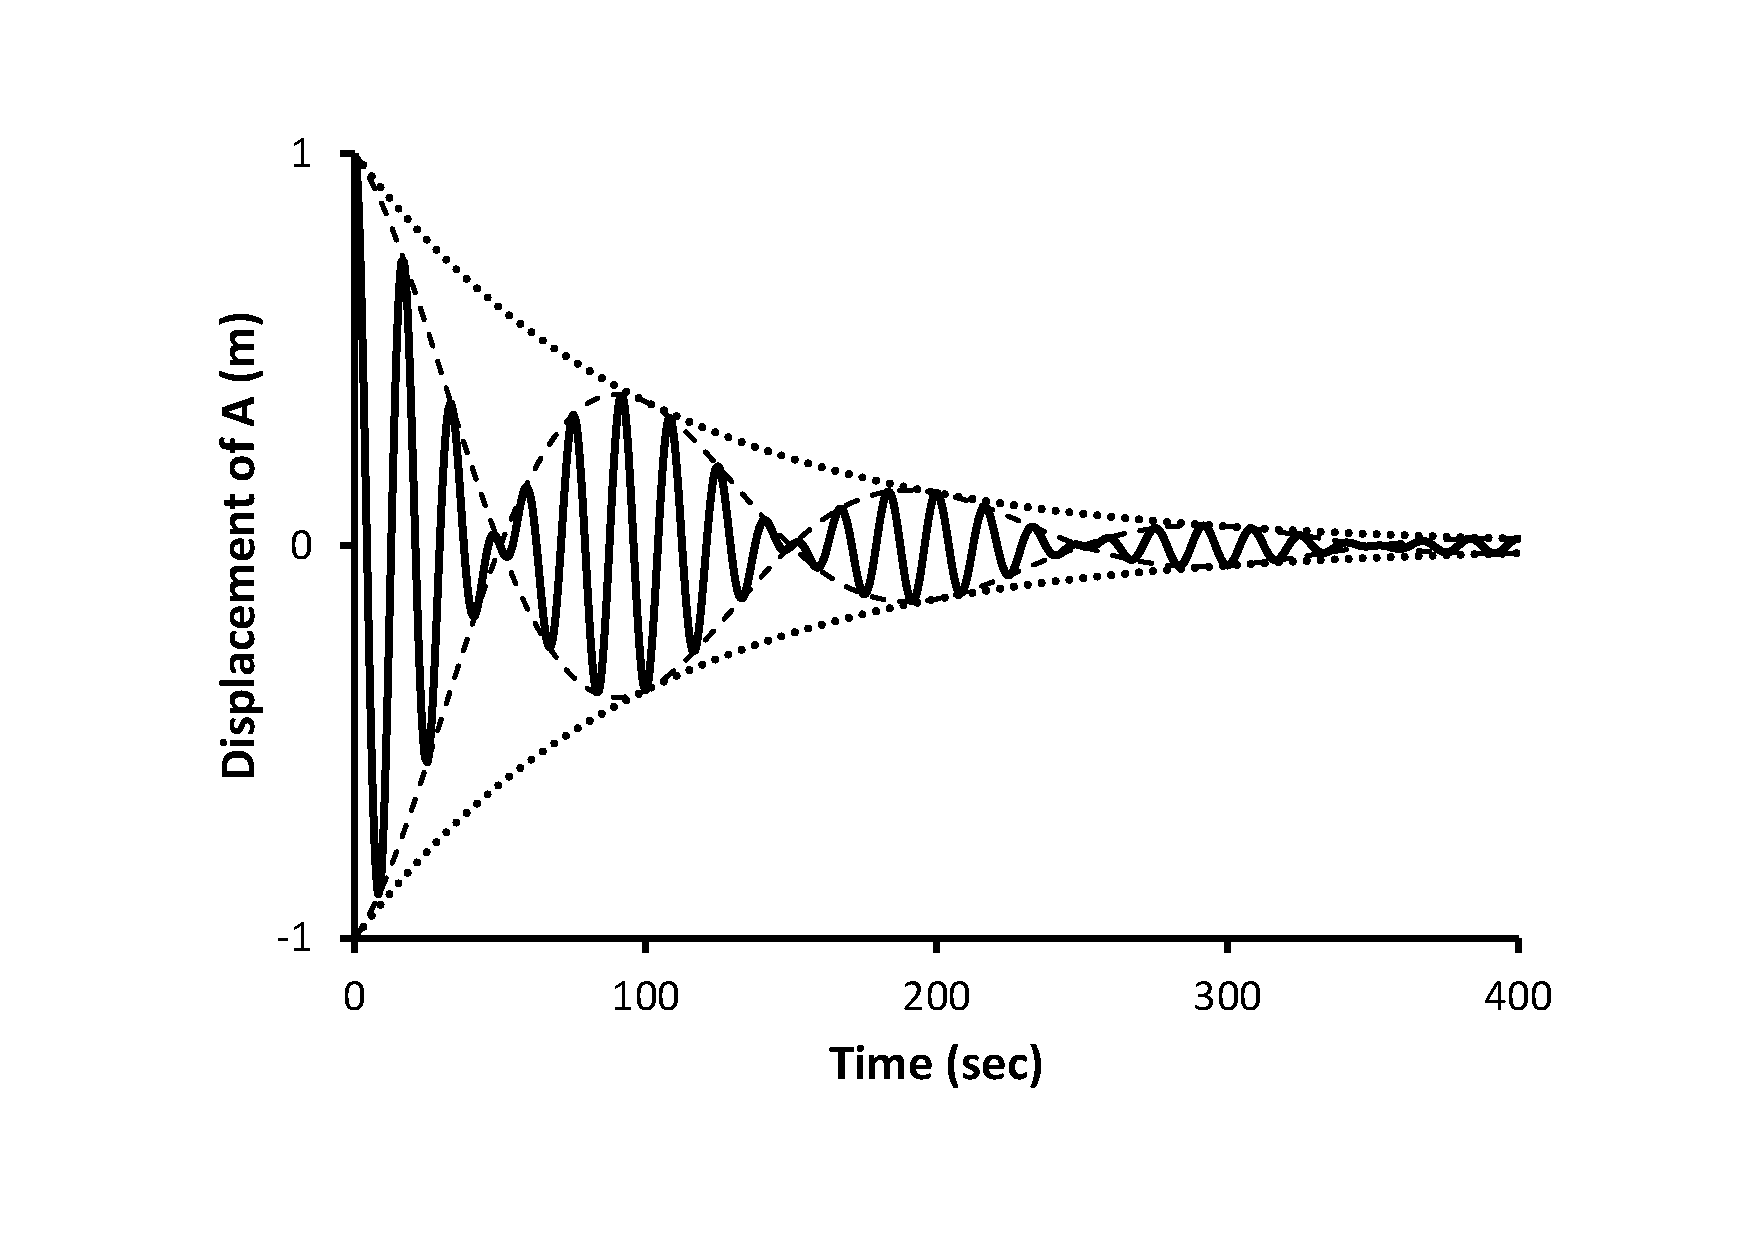
\includegraphics[width=9cm]{Figure01.pdf}
\end{center}
\caption{{\bf Magnetization as a function of applied field.} Note that ``Fig.'' is abbreviated. There is a period after the figure number. It is good practice to explain the significance of the figure in the caption.}
\label{Fig01}
\end{figure}



\subsection{References}

Number citations consecutively in square brackets \cite{True00}. The sentence punctuation follows the brackets \cite{Schluter00}. Multiple references \cite{Schluter00}, \cite{Plazzo11} are each numbered with separate brackets \cite{True00,Schluter00,Plazzo11}. When citing a section in a book, please give the relevant page numbers \cite{Schluter00}. In sentences, refer simply to the reference number, as in \cite{Plazzo11}. Do not use ``Ref. \cite{Plazzo11}'' or ``reference \cite{Plazzo11}'' except at the beginning of a sentence: ``Reference \cite{Plazzo11} shows ... .''

References should be written to the following formats:

Authors should be listed surname first, followed by a comma and initials of given names. Titles of articles cited in reference lists should be in upright, not italic text; the first word of the title is capitalized, the title written exactly as it appears in the work cited, ending with a full stop. Book titles are italic with all main words capitalized. Journal titles are italic and abbreviated according to common usage. Volume numbers are bold. The publisher and city of publication are required for books cited. References to web-only journals should give authors, article title and journal name as above, followed by URL in full or DOI if known. References to websites should give authors if known, title of cited page, URL in full, and year of posting in parentheses. The year of publication (posting) should written in parentheses.

\subsection{Abbreviations and Acronyms}

Define abbreviations and acronyms the first time they are used in the text, even after they have already been defined in the abstract.

\subsection{Equations}

Number equations consecutively with equation numbers in parentheses flush with the right margin, as in (\ref{eq01}). First use the equation editor to create the equation. Then select the ``Equation'' markup style. Press the tab key and write the equation number in parentheses. To make your equations more compact, you may use the solidus ( / ), the exp function, or appropriate exponents. Use parentheses to avoid ambiguities in denominators. Punctuate equations when they are part of a sentence, as in
\begin{equation}\label{eq01}
\begin{split}\int_0^{r_2} &F(r,\varphi)\,dr\,d\varphi=[\sigma r_2 /(2\mu_0 )] \\
&\times\int_0^{\infty} \exp(-\lambda |z_j -z_i |)\lambda^{-1} J_1 (\lambda r_2 )J_0 (\lambda r_i )d\lambda.\end{split}
\end{equation}

Be sure that the symbols in your equation have been defined before the equation appears or immediately following. Refer to ``(\ref{eq01}),'' not ``Eq. (\ref{eq01})'' or ``equation (\ref{eq01}),'' except at the beginning of a sentence: ``Equation (\ref{eq01}) is ... .''

%\subsection{Theorems}
%\begin{thm}
%\end{thm}
%\begin{defn}
%\end{defn}

\subsection{Other Recommendations}

Use one space after periods and colons. Hyphenate complex modifiers: ``zero-field-cooled magnetization.''

Use a zero before decimal points: ``0.25,'' not ``.25.'' Use ``$\rm cm^3$,'' not ``cc.'' Indicate sample dimensions as ``$0.1\,\rm cm\times 0.2\, cm$,'' not ``$0.1\times 0.2\,\rm cm^2$.'' The abbreviation for ``seconds'' is ``s,'' not ``sec.'' Do not mix complete spellings and abbreviations of units: use ``Wb/m'' or ``wevers per square meter,'' not ``webers/m.'' When expressing a range of values, write ``7 to 9'' or ``7-9,'' not ``7$\sim$9.''

A parenthetical statement at the end of a sentence is punctuated outside of the closing parenthesis (like this). (A parenthetical sentence is punctuated within the parentheses.) In American English, periods and commas are within quotation marks, like ``this period.'' Other punctuation is ``outside''!

If you wish, you may write in the first person singular or plural and use the active voice (``I observed that ...'' or ``We observed that ...'' instead of ``It was observed that ...'').

\section{CONCLUSION}

Abstracts and Papers should be written according to the following order: ①Title ②Abstract ③Main text ④References.

\begin{thebibliography}{99}
\bibitem{True00} True, H. L. and Lindquist, S. L. A. A yeast prion provides a mechanism for genetic variation and phenotypic diversity. {\it Nature} {\bf 407}, 477--483 (2000)
\bibitem{Schluter00} Schluter, D. {\it The Ecology of Adaptive Radiation} (Oxford Univ. Press, 2000)
\bibitem{Plazzo11} Plazzo, A. P. et al. Bioinformation and mutational analysis of channelrhodopsin-2 cation conducting pathway. {\it J. Biol. Chem.} http://dx.doi.org/10.1074/jbc.M111.326207 (2011)
\end{thebibliography}







\end{document}